
%(BEGIN_QUESTION)
% Copyright 2015, Tony R. Kuphaldt, released under the Creative Commons Attribution License (v 1.0)
% This means you may do almost anything with this work of mine, so long as you give me proper credit

In this system a loop controller receives a process variable signal from a 2-wire (loop-powered) transmitter, and sends its own 4-20 mA control signal to operate a control valve.  A data acquisition unit (DAQ) performs the auxiliary function of monitoring the process variable signal (voltage dropped across the loop resistor) and reporting it over a digital network where it is recorded on the hard drive of a personal computer.  If it helps, you may think of a DAQ as being nothing more than a multi-channel voltmeter, sensing voltage between each of its input terminals ({\tt In\_1}, {\tt In\_2}) and its ``common'' ({\tt Com}) terminal:

$$\includegraphics[width=15.5cm]{i02557x01.eps}$$

Unfortunately, the DAQ not only registers the DC signal value, but also any HART pulses present in the transmitter circuit whenever a technician connects a HART communicator to the transmitter to do any maintenance work.  The operators are annoyed by the misleading ``noise'' on the DAQ-recorded signal whenever a technician does routine work on that transmitter, and so they come to you asking for a solution.

\vskip 10pt
 
Devise a simple modification to this circuit that will eliminiate (or at least minimize) the ``HART noise'' seen by the DAQ without impeding its ability to record normal process variable signal values.

\vskip 20pt \vbox{\hrule \hbox{\strut \vrule{} {\bf Suggestions for Socratic discussion} \vrule} \hrule}

\begin{itemize}
\item{} A useful problem-solving technique is to sketch a simple diagram of the system you are asked to analyze.  This is useful even when you already have some graphical representation of the problem given to you, as a simple sketch often reduces the complexity of the problem so that you can solve it more easily.  Draw your own sketch showing how the given information in this problem inter-relates, and use this sketch to explain your solution.
\item{} A useful analytical technique for any DC electric circuit is to identify all electrical sources and loads in the circuit, annotate the diagram with arrowheads showing the directions of all currents, and also with ``+'' and ``$-$'' symbols (and/or curved arrows) showing the polarities of all component voltages.  Show how this helps you analyze the circuit shown in this question.
\end{itemize}

\underbar{file i02557}
%(END_QUESTION)





%(BEGIN_ANSWER)


%(END_ANSWER)





%(BEGIN_NOTES)

A simple resistor-capacitor low-pass filter connected between the resistor and the DAQ channel will suffice:

$$\includegraphics[width=15.5cm]{i02557x02.eps}$$

The values of $R$ and $C$ should be chosen to create a cutoff frequency lower than the lowest frequency expected with HART (1200 Hz), but not so low that relevant changes in the process variable would be excessively damped.

\vskip 10pt

Beware of any solutions that would shunt HART signals around the 250 ohm loop resistance, such as a capacitor connected in parallel with DAQ input!  This would solve the HART interference problem, but at the cost of impeding all HART communication!

%INDEX% Basics, 2-wire loop-powered transmitter: connection to process controller

%(END_NOTES)


